\documentclass{standalone}
\usepackage{tikz,calc}
\usetikzlibrary{intersections, calc}
\renewcommand{\familydefault}{\sfdefault}

\tikzstyle{level}=[thick, opacity = .93, black]
\begin{document}
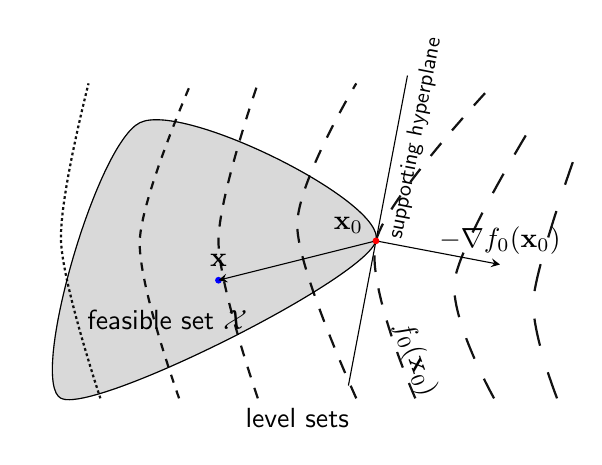
\begin{tikzpicture}[>=stealth]
  % \draw [fill = blue, opacity = .3] plot [smooth cycle] coordinates {(0,0) (1,1) (2,1) (3,-1) (0,-1)};
  % \draw [fill = red, opacity = .3] plot [smooth cycle] coordinates {(2,0) (3,2) (4, 1.5) (4, -1)};
  \draw [fill = gray, opacity = .3] plot [smooth cycle] coordinates {(0,2.5) (3,1) (-1, -1)};
  \draw [draw = black] plot [smooth cycle] coordinates {(0,2.5) (3,1) (-1, -1)};

  % \draw plot [smooth cycle] coordinates {(0,0) (1,1) (2,1) (3,-1) (0,-1)};

  \draw [level, dash pattern=on 1pt off 1pt] plot [smooth] coordinates {(-0.5, -1) (-1, 1) (-0.65, 3)};
  \draw [level, dash pattern=on 3pt off 3pt] plot [smooth] coordinates {(0.5, -1) (0, 1) (0.65, 3)};
  \draw [level, dash pattern=on 4pt off 4pt] plot [smooth] coordinates {(1.5, -1) (1, 1) (1.5, 3)};
  \draw [level, dash pattern=on 5pt off 5pt] plot [smooth] coordinates {(2.75, -1) (2, 1.2) (2.75, 3)};
  \draw [level, dash pattern=on 6pt off 6pt] plot [smooth] coordinates {(3.5, -1) (3, 1) (4.5, 3)};
  \draw [level, dash pattern=on 8pt off 8pt] plot [smooth] coordinates {(4.5, -1) (4, .5) (5, 2.5)};
  \draw [level, dash pattern=on 10pt off 10pt] plot [smooth] coordinates {(5.3, -1) (5, .25) (5.5, 2)};


  \node at (2.65, 1.2) {$\mathbf{x}_0$};
  \node at (0.35, 0) {feasible set $\mathcal{X}$};
  \node at (2, -1.25) {level sets};
  \def\k{5.25}
  \def\ax{2.65}
  \def\bx{3.4}
  \def\ay{\d*(\ax - 3) + 1}
  \draw ({\ax}, {\k*(\ax - 3) + 1})  --  ({\bx}, {\k*(\bx - 3) + 1});
  \draw [->] (3, 1)  --  (3 + .3*\k, 1 - .3);
  \node at (3 + .3*\k, 1) {$-\nabla f_0(\mathbf{x}_0)$};
  \node at (1, .75) {$\mathbf{x}$};
  \draw [fill = blue, draw = blue] (1, .5 ) circle (1pt);
  \draw [->] (3, 1)  --  (1, .5);
  \node [rotate = -70] at (3.5, -.5) {$f_0(\mathbf{x}_0)$};

  \draw [fill = red, draw = red] (3, 1 ) circle (1pt);
  \node [scale = .8, rotate = 79] at (3.5, 2.3) {supporting hyperplane};
\end{tikzpicture}
\end{document} 